\documentclass[oneside, a4paper, 12pt, titlepage]{article}
\usepackage[ngerman]{babel}
\usepackage{graphicx}
\usepackage[usenames, dvipsnames]{xcolor}
\usepackage[utf8]{inputenc}
\usepackage[T1]{fontenc}
\usepackage{listings}
\usepackage{hyperref}

\title{Information Retrieval: MSDS Search Report}
\date{ \small{Institut für Informatik, Universität Leipzig} \\[2ex] September 2018}
\author{Adrian Fichtner, Leonard Krause, Salomo Pflugradt, David Reinartz}
\begin{document}

\flushbottom
\maketitle
\tableofcontents
\newpage

\section{Domain}
Bei dem vorliegenden Datensatz handelt es sich um eine Sammlung von sogenannten ``Material Safety Data Sheets'' (kurz MSDS).
Diese beinhalten Informationen zu von der NATO anerkannten ''Produkten standardisierter Materialversorgung''.
Sie werden meist von Fachleuten zur Einschätzung von Gefahren und für Informationen zum richtigen Umgang herangezogen.
Die ca. 235,000 Datenblätter stammen von \textit{hazard.com} und werden von Amazon AWS zum Download bereitgestellt.
\subsection{Motivation}
MSDS spielen in vielen Bereichen eine große Rolle für die Sicherheit aller Beteiligten. In nahezu allen Berufsfeldern, aber auch im privaten Umfeld können durch das Befolgen der Sicherheitsinformationen die Gesundheit der eigenen Person und anderer Menschen sowie das Wohlergehen der Natur gesichert werden. Oft sind diese Informationen jedoch in dicken Papierordnern versteckt oder sogar gar nicht vorhanden, was die schlechte Gewohnheit fördert sich die Informationen nicht noch einmal vor Augen zu führen und so ein potentielles Sicherheitsrisiko birgt. Mit dieser Suchmaschine soll eine einfache, schnelle und bequeme Möglichkeit geboten werden an die richtigen Informationen zu gelangen, sodass die Sicherheit der Anwender gewährt ist. Es werden mit diesem Projekt zwei Fälle betrachten:

1.) Der Nutzer befindet sich in einer Notsituation und benötigt schnell Hilfe. Er hat z.B. eine gefährliche Flüssigkeit verschüttet, weswegen nur noch Zeit bleibt den Namen des Produkts und des Herstellers auf der Flasche zu lesen. In diesem Fall sollte die \textit{General Search} Funktionalität genutzt werden.

2.) Der Nutzer hat viel Zeit und alle nötigen Informationen.
Er möchte z.B. ein neues Produkt kaufen und sich im Vorhinein über eventuelle Sicherheitshinweise informieren. Dazu bietet die Suchmaschine eine \textit{Advanced Search} Funktionalität mit der die gewünschten Bereiche im Datenblatt direkt adressiert werden können.
\subsection{Struktur der Dokumente}
Die Struktur von MSDS variiert je nach Herkunftsland und den dort geltenden Richtlinien. Da der vorliegende Datensatz jedoch komplett aus amerikanischen MSDS besteht, ist die grobe Struktur der Blätter im Wesentlichen gleich. Im Idealfall ist ein MSDS wie in Abb. \ref{dia1} (mittlere Spalte) zu sehen aufgebaut. Nach kurzer Untersuchung des Datensatzes war jedoch zu erkennen, dass viele der Dokumente dieser Aufteilung nicht folgen. Durch das später beschriebene Indizieren der Dokumente in Solr konnte mit der Query
\begin{center}\texttt{-<fieldName>:[* TO *] \&\& docType:datasheet} \end{center}
die Zahl der Dokumente gefunden werden, bei denen die jeweilige Kategorie \texttt{<fieldName>} leer ist (siehe Abb. \ref{dia1}, linke Spalte). Es fällt auf, dass fünf der sechs letzten Kategorien bei ca. 55,000 Dokumenten fehlen. Der Betrag von der Schnittmenge der Dokumente, bei denen diese Kategorien fehlen ist 52861. Somit ist zu vermuten, dass diese Dokumente aus einem separaten Teildatensatz stammen, welcher mit den übrigen Daten zusammengeführt wurde.
In jeder Textdatei sind die einzelnen Kategorien durch mehrere Gleichheitszeichen mit in der Mitte aufgeführter Kategoriebezeichnung getrennt.
Als Vorarbeit wurden mithilfe kleiner Python Skripte fehlende Kategoriebezeichnungen hinzugefügt, fälschlich als Überschrift markierte Zeilen entfernt und ein Disclaimer am Ende jedes Dokumentes entfernt. Der Disclaimer wird nun auf der Website angezeigt.
Durch die recht uneinheitliche Strukturierung hat es sich als Herausforderung erwiesen, die Daten in geeignete Java Objekte (POJOs) zu übertragen.
Wir haben uns entschieden, wichtige Daten (z.B. Name des Produkts, Kennzahlen) in eigenen Attributen zu speichern um gezielter Suchen zu können (siehe Abb. \ref{dia1}).
Dies hat sich besonders bei der Advanced Search und der beteiligten Autocompletion als Vorteil herausgestellt. Zudem wurden die Inhalte aller vorhandenen Kategorien als Volltext gespeichert um das MSDS dem User korrekt formatiert präsentieren zu können und eine Suche im gesamten Dokument zu ermöglichen.
Zusätzlich kann jedes Produkt mehrere Zutaten mit den eigenschaften CAS-Nummer und Name besitzen. Diese werden dem POJO als Liste von Ingredient-Objekten hinzugefügt und automatisch von Solr korrekt gemapped (lediglich die Query muss angepasst werden, siehe Suche).
\subsection{Anreicherung}
Nach weiterer Recherche hat sich gezeigt, dass die FSC Nummer für Faceting genutzt werden kann. Die vierstellige Kennzahl unterteilt die Produkte in Federal Supply Groups (Ziffern 1 \& 2) und Federal Supply Classes (Ziffern 1 - 4). Es handelt sich dabei um Kategorien zur Klassifizierung von Materialien. Mithilfe von zuvor aus dem Internet abgerufenen Informationen wird während des Erstellens der POJOs durch die FSC auf die FSG geschlossen und schließlich werden beide Kennzahlen zu ihren Beschreibungen gemapped. Dies ermöglicht zum einen zweistufiges Faceting und zum anderen besseres Retrieval durch präzisere Informationen.
\begin{figure}[!p]
\centering
\caption{MSDS Struktur/Java Object} \label{dia1}
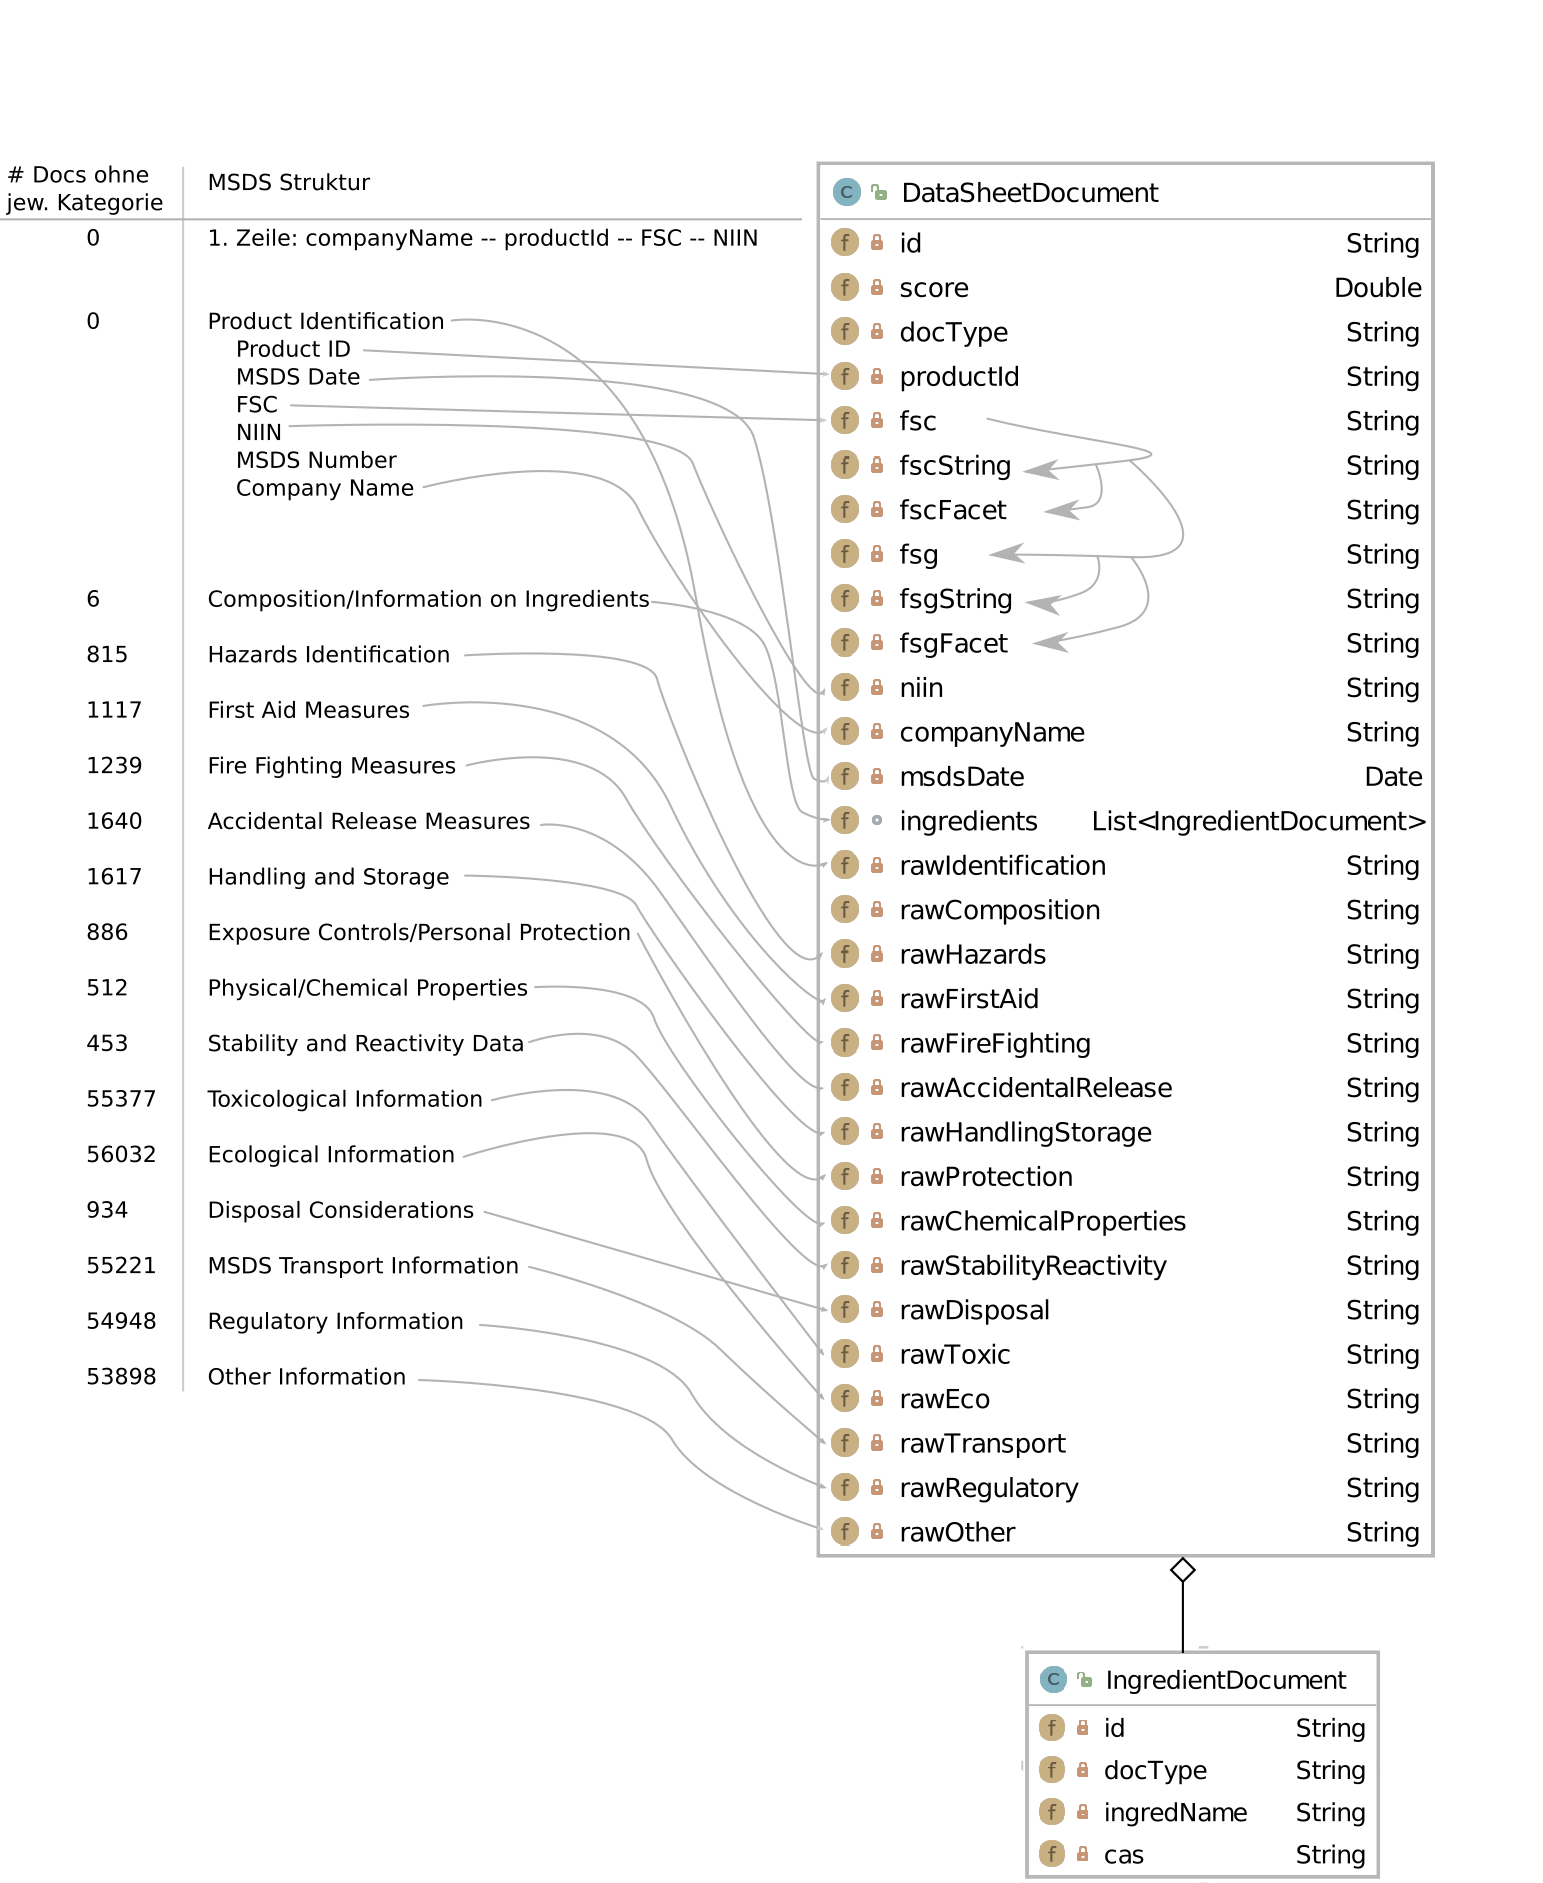
\includegraphics[scale=0.9]{dia1b.png}
\end{figure}
\pagebreak

\section{Architektur}
\begin{figure}[!ht]
\caption{Architektur der Suchmaschine} \label{dia2}
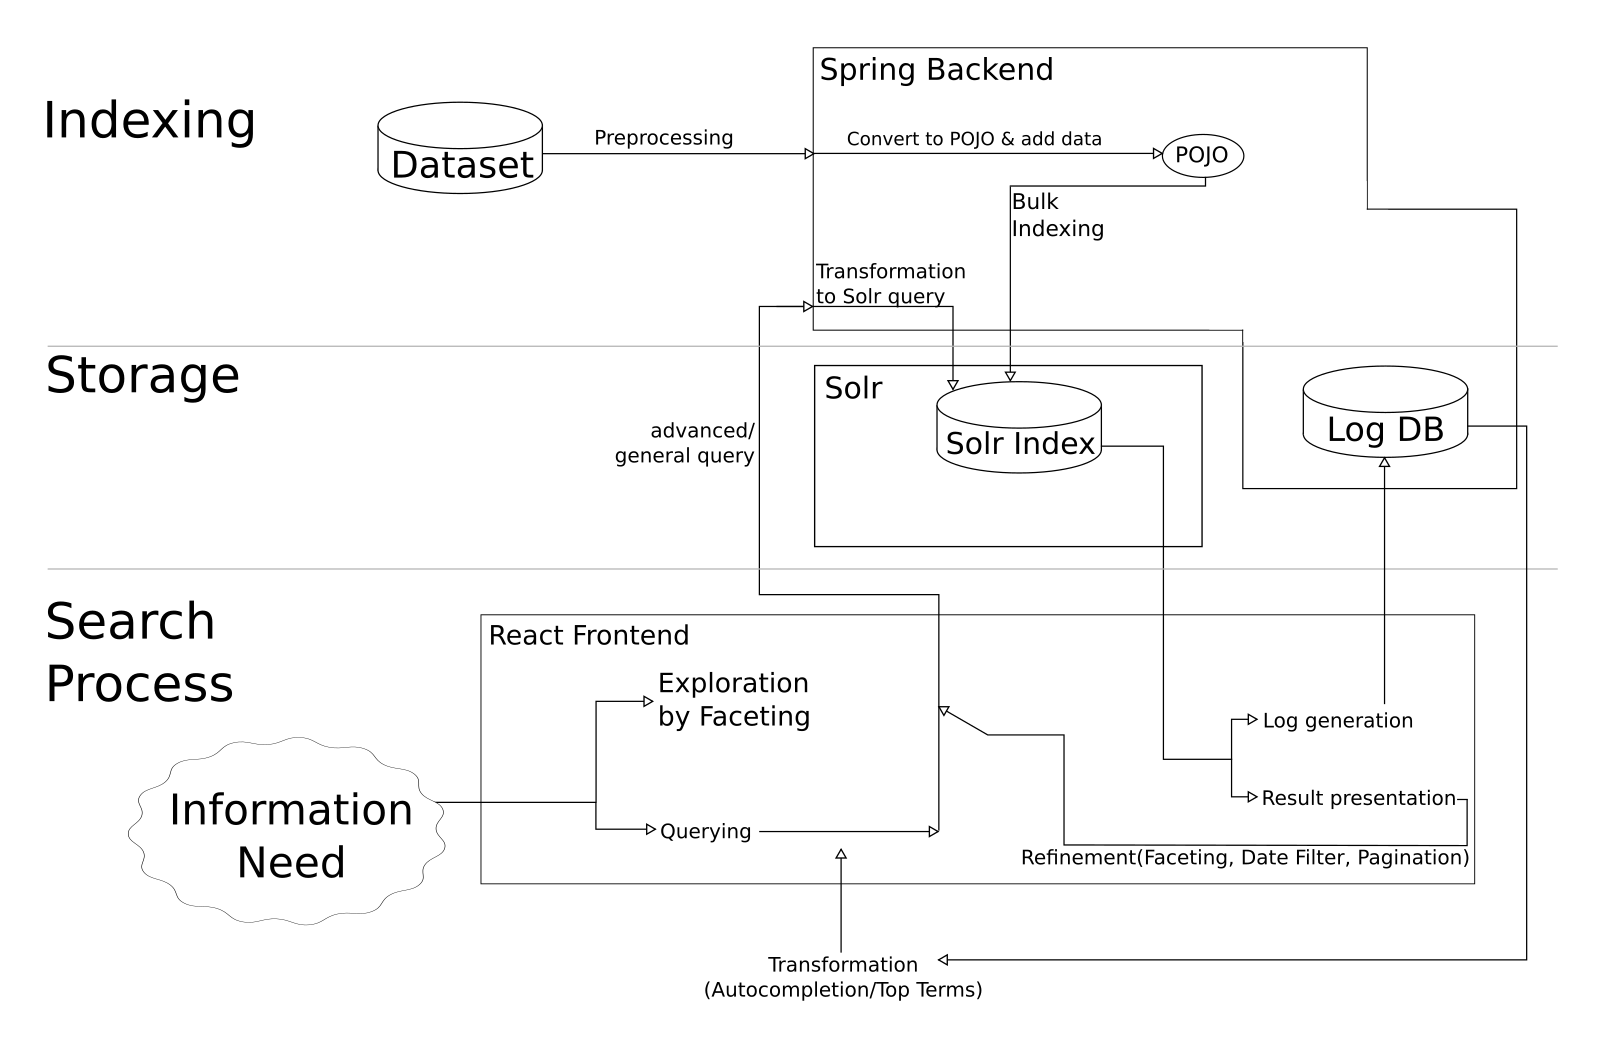
\includegraphics[scale=0.45]{dia2_svg.png}
\end{figure}

\subsection{Technologie}
Das Backend ist in \textit{Java} geschrieben und nutzt das \textit{Spring} Framework. Die gewählte Suchplattform ist \textit{Solr} und ist mit Spring über das \textit{spring-data-solr} Modul verbunden. Spring ermöglicht mit dieser Integration eine recht einfache (wenn auch nicht immer bestmögliche) Lösung, um ein robustes Backend aufzubauen, mit Solr zu kommunizieren, Endpoints bereitzustellen und Logs in einer Datenbank zu speichern.
Für letzteres wird \textit{MariaDB} verwendet. Innerhalb des Backends wird auf eine klare Mehrebenenarchitektur wertgelegt (Solr $\Leftrightarrow$ Repository/Solr API $\Leftrightarrow$ Service $\Leftrightarrow$ Controller $\Leftrightarrow$ Frontend).
Die Kommunikation mit dem Frontend findet über \textit{JSON} statt und ist in einer \textit{OpenAPI Specification (Swagger)} dokumentiert.
Das Frontend nutzt für eine moderne, responsive Darstellung die JavaScript Library \textit{React} und das Framework \textit{Material-UI}. Die Datenhaltung im Frontend erfolgt mittels eines globalen \textit{Redux} Stores.
Automatisierte Builds, mit anschließendem Deployment (CI/CD) werden von \textit{Jenkins} unter Verwendung von \textit{Docker} und \textit{Ansible} ausgeführt.
Dies ermöglicht neben einer laufenden Demo-Instanz vom \texttt{develop}-Branch auch das leichtes Aufsetzen des Programms auf dem eigenen PC.
Der indizierte Datensatz und die Log-Datenbank werden in einem Docker-Volume gespeichert, sodass bei einem Neustart der Anwendung die Indizierung nicht jedes Mal von Neuem beginnt und die Logs erhalten bleiben. Datenbankmigrationen der Log-Datenbank von einer Version zur nächsten, werden mit Flyway verwaltet.\\
In Abb. \ref{dia2} ist die Architektur der Suchmaschine in Anlehnung an die Abbildung aus der Vorlesung grob dargestellt. Sie beschreibt den Indizierungsprozess, sowie den Suchprozess. Der Nutzer kann seinen Information Need durch Exploration oder Querying stillen. Die Queries können verfeinert werden und das Nutzerverhalten wird in Logs gespeichert.

\subsection{Backend}
\subsubsection{Indizierung}
Nach der Umwandlung der Daten in POJOs findet der eigentliche Indizierungsprozess statt. Es werden 5 Solr Feldtypen verwendet, welche zum Großteil auf Solr Standardfeldtypen basieren und in Tabelle \ref{analyzer} dargestellt sind. (\textcolor{OliveGreen}{Grün gefärbte} Analyzer weichen von den Standardtypen ab und wurden selbst gewählt.)
\begin{table}[!ht]
\caption{Analyzers}
\label{analyzer}
\begin{tabular}{|l|l|l|}
\hline
Felder & Feldtyp & Analyzer \\ \hline
 \begin{tabular}{l}
 fsgFacet \\
 fscFacet \\
 fsg
 \end{tabular}
 & \texttt{string} & $-$ \\ \hline
 \begin{tabular}{l} msdsDate \end{tabular} & \texttt{pdate} & $-$ \\ \hline
 \begin{tabular}{l}
 fsc\\
 niin\\
 cas
 \end{tabular} & \texttt{string\_mod} & \hspace{0.5mm} \textcolor{OliveGreen}{Edge-N-Gram-Filter} \\ \hline
 \begin{tabular}{l} 
 productId \\
 fscString \\
 fsgString \\
 companyName \\
 ingredName
 \end{tabular} 
 & \texttt{text\_en\_splitting\_mod} & \begin{tabular}{l} Whitespace Tokenizer $\rightarrow$ \\ Stopword-Removal $\rightarrow$ \\ Tokenizer (word delimiter) $\rightarrow$ \\ LowerCaseFilter  $\rightarrow$ \\ Porter-Stemmer \\ (only while indexing) $\rightarrow$ \\ \textcolor{OliveGreen}{Edge-N-Gram-Filter} \end{tabular} \\  \hline
 \begin{tabular}{l}
 rawIdentification \\
 rawComposition \\
 ... \\
 rawOther
 \end{tabular}
 & \texttt{text\_en\_raw\_mod} & \begin{tabular}{l} \textcolor{OliveGreen}{Classic Tokenizer} $\rightarrow$ \\ \textcolor{OliveGreen}{Lower-Case-Filter} $\rightarrow$ \\
 \textcolor{OliveGreen}{Stopword-Removal} $\rightarrow$ \\ \textcolor{OliveGreen}{Porter-Stemmer} \end{tabular} \\
 \hline
\end{tabular}
\end{table}

Die Felder fscFacet, fsgFacet, fsg und msdsDate werden nicht analysiert, da keine Verwendung für weitere Tokens besteht.
Für die Hauptfelder wurde der Solr-Feldtyp \texttt{text\_en\_splitting} gewählt, da er neben agressiver Tokenisierung auch mehrere Varianten der Tokens speichert (``paint-remover'' -> ``paint'', ``remover'', ``paintremover'').
Er ist also perfekt für Felder geeignet, die kurze Informationen wie Firmennamen und Produktbezeichnungen beinhalten.
Die Solr-Feldtypen \texttt{string} und \texttt{text\_en\_splitting} wurden je um einen Edge-N-Gram-Filter erweitert, durch den 1-Gramme bis 15-Gramme von der linken Seite des Tokens aus erzeugt werden.
Dadurch entsteht zum einen die Möglichkeit mit eingegeben Teilworten ein Match zu erlangen, andererseits werden Suggestions ermöglicht (siehe \ref{Suggestions}, Suggestions).
Zuletzt wurde für die Volltextsuche ein eigener Feldtyp erstellt, welcher als Hauptelement eine speziell angepasste Stoppwortliste enthält, sodass die Attributbezeichnungen gefiltert werden, während die Attributwerte bestehen bleiben.
Die ``Ingredients''-Listen werden nach Standard-Solr-Vorgehen im gleichen Index wie die Datasheets gespeichert und unterscheiden sich durch das Attribut docType (entweder ``datasheet'' oder ``ingredient'').


\subsubsection{Suche}
Wie in der Motivation angedeutet haben Nutzer zwei Möglichkeiten die Suchmaschine zu nutzen:
\paragraph{General Search (\(/search\))}
Nachdem der Nutzer einen Search Term in das Feld eingegeben und die Suche gestartet hat, wird der Term analysiert und daraus eine Solr-Query generiert. Diese wird abgeschickt und dem Nutzer werden die Ergebnisse präsentiert. Die Such-Pipeline wird in Abb. \ref{dia3} dargestellt.
\begin{figure}[!ht]
\caption{Suchpipeline für General Search} \label{dia3}
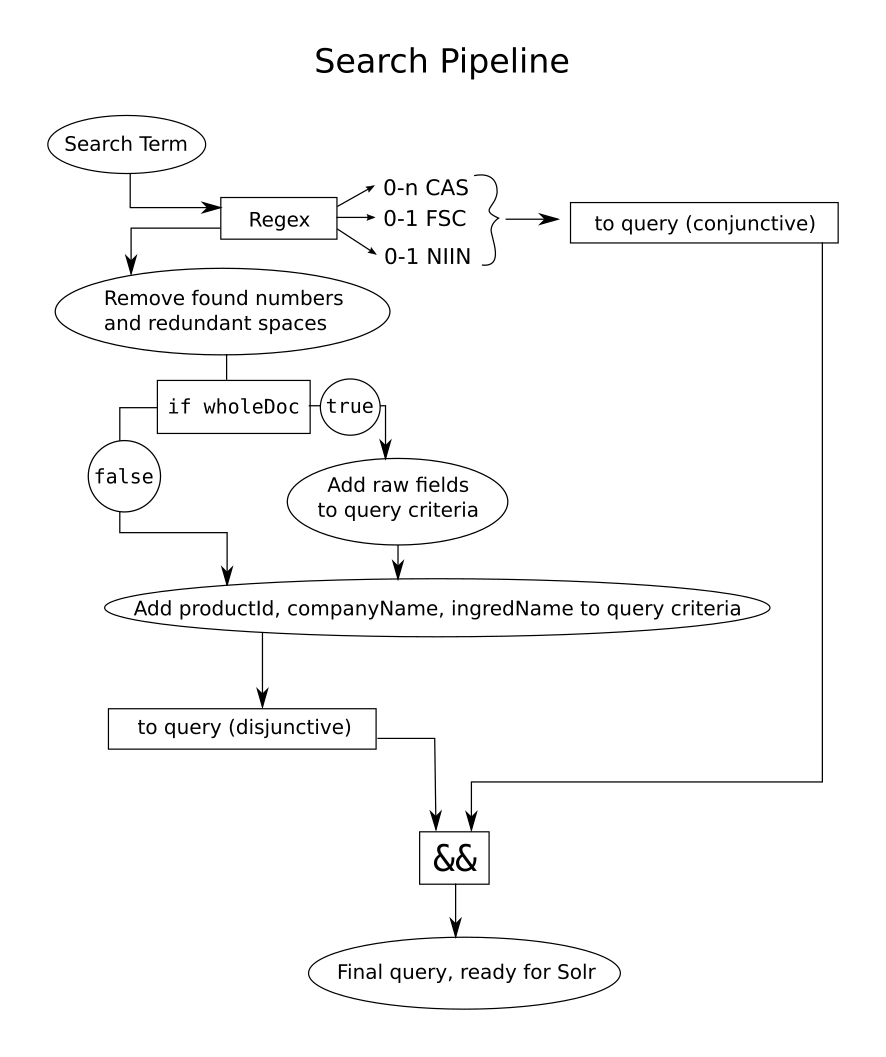
\includegraphics[scale=0.7]{dia3_svg.png}
\end{figure}
Zunächst werden etwaige Kennzahlen per Regex erkannt, herausgefiltert und aus ihnen eine konjunktive Solr-Query erstellt. Befindet sich ein Ausrufezeichen vor einer der Zahlen, so wird die Query invertiert und es werden Dokumente gefunden, die den gegebenen Wert nicht beinhalten. Danach werden die Kennzahlen aus dem Term entfernt und er wird gesäubert.
Soll im gesamten Dokument gesucht werden, werden nun Queries für die wichtigen Kennfelder \textit{und} die Volltextfelder erzeugt (z.B. \texttt{rawIdentification}), ansonsten werden \textit{nur} Queries für die Kennfelder generiert.
Diese erzeugten Queries werden nun per Konjunktion mit der oben genannten Query zusammengefügt und zur Suche an Solr geschickt.
Durch die automatische Erkennung der Kennzahlen wird die Suche für den Nutzer verbessert, ohne dass er besonders darauf achten muss. Wird bspw. nur eine CAS Nummer eingegeben, so wird direkt im CAS Feld gesucht und der Nutzer erhält präzisere Ergebnisse.
\paragraph{Advanced Search (\(/advancedSearch\))}
Die Advanced Search ist wesentlich simpler als die General Search, da die gegebenen Suchbegriffe schon Kategorien zugeordnet sind.
Für jedes nicht-leere Feld wird eine Query erzeugt -- eventuell invertiert -- und diese werden als Konjunktion zusammengefügt. In der entstandenen Query sind dann verpflichtende Werte gegeben, die für einen Match mit einem Dokument existieren müssen. Zudem können bei der Advanced Search die Dokumente durch Datumsangaben gefiltert werden. Diese Funktion existiert nur bei dieser Suchart, da der Nutzer bei der General Search nicht ein bestimmtes Datenblatt sucht, sondern generelle Information zu dem Produkt. Volltextsuche hingegen gibt es bei der Advanced Search nicht (siehe \ref{wds} Whole Document Search).

Als weitere Hürde hat sich das Zusammenfügen von Kind- und Elterndokumenten nach dem Suchen erwiesen, welche jedoch durch Mitgabe einer Fieldlist (\texttt{\{"*", "[child parentFilter=docType:datasheet]"\}}
) leicht zu überwinden war.

\subsubsection{Weitere Funktionalitäten}

\paragraph{2-Stufen Faceting}
Die Anreicherung des Datensatzes mit Informationen zu FSC und FSG ermöglicht die Bereitstellung einer Faceting Funktion. So hat der Nutzer die Möglichkeit seine Suche effektiv zu Verfeinern. Auch kann nach Betätigen des Suchknopfes ohne vorherige Eingabe eines Suchbegriffs der gesamte Datensatz erkundet werden. Das Faceting findet zweistufig statt, da die oben genannte Struktur der FSC Nummer dies anbietet. Der Nutzer wählt zunächst eine FSG (z.B. ``80'' für die Gruppe ``Brushes, Paints, Sealers and Adhesives'') und danach eine FSC aus dieser Gruppe (z.B. ``8030'' für die Klasse ``Preservative and Sealing Compounds''). Sucht er Beispielsweise nach Goldfarbe und gibt deswegen ``gold'' ein, so erhält u.a. 280 Dokumente aus der Gruppe ``Chemicals and Chemical Products'' und 275 Dokumente aus der Gruppe ``Brushes, Paints, Sealers and Adhesives'' (insg. 988 Ergebnisse). Da er nach Farbe sucht, kann er nun das Result Set um gut zwei Drittel verkleinern, indem er auf letztere Gruppe klickt.

\paragraph{Suggestions (\(/suggest\))} \label{Suggestions}
Suggestions gibt es momentan nur bei der Advanced Search. Diese Funktionalität kann realisiert werden, da bei der Indizierung N-Gramme von links erzeugt werden. Gibt der Nutzer z.B. ``Exx'' als Company Name ein, so liefert der Suggestion Service die top Ergebnisse für diese Suche - es werden alle Dokumente gematched, die im Feld companyName ein Token mit dem Präfix ``Exx'' haben - und schlägt sie dem Nutzer vor. Das bedeutet natürlich, dass es sich bei den vorgeschlagenen Werten um exakte Attributwerte handelt, so wie sie in den Dokumenten stehen. Dies ist bei Kennzahlen offensichtlich sinnvoll, da man nur nach einer Zahl suchen möchte, die auch existiert. Bei den übrigen Kennfeldern kann dies jedoch auch von Vorteil sein, da z.B. direkt gesamte Firmennamen angezeigt werden - was bei der Advanced Search Zeit sparen kann.

\paragraph{Fuzzy}
Wird Fuzzy Search aktiviert, so wird für die Textfelder an jeden Suchterm in der Solr-Query ein ``\texttt{$\sim$1}'' konkateniert. Bei Zahlfeldern geschieht dies nicht, da aus der Ähnlichkeit zweier Zahlen nicht unbedingt deren ähnliche Bedeutung folgt. In der Evaluation wird bewertet wie sinnvoll Fuzzy Search in diesem Kontext ist und ob es die MAP verändert.

\paragraph{Whole Document Search} \label{wds}
Die Suche im gesamten Dokument gibt es nur bei der General Search, da bei der Advanced Search die Felder in denen gesucht wird schon zuvor feststehen. Wird die Volltextsuche aktiviert so wird zusätzlich zu den Kennfeldern in allen Volltextfeldern nach den gegebenen Begriffen gesucht.
Da während des Indizierens alle Worte entfernt werden, die im Datensatz in mehr als ca. 150,000 Dokumenten vorkommen, kann durch eine Kombination von zwei Suchtermen im Idealfall die Schnittmenge schon auf 65,000 Dokumente reduziert werden.
Auch inwiefern die Volltextsuche das Retrieval beeinflusst wird in der Evaluation bewertet.

\label{logging}
\paragraph{Logging (\(/logging\) und \(/top\))}
Das Frontend stellt pro Suchanfrage des Nutzers ein Log Objekt zusammen und sendet dieses anschließend an das Backend. Mithilfe von 3 Timestamps, werden zunächst 2 Zeiträume getrackt. Der erste Zeitraum beginnt mit dem Absenden der Suchanfrage und endet, wenn die Ergebnisse am Frontend ankommen und dem Nutzer angezeigt werden. Mit dieser Zeitspanne wird gemessen, wie lange der Nutzer effektiv auf Ergebnisse warten muss. Falls diese Zeitspanne zu groß wird, muss entweder die Performance des Backends optimiert werden, oder die Menge der übetragenen Daten reduziert werden. Der zweite Zeitraum beginnt mit dem Ende des ersten und endet, wenn der Nutzer die Suchanfrage abschließt. Eine Suchanfrage gilt als abgeschlossen, wenn der Nutzer eine neue Suchanfrage absendet, oder die Suche schließt. Die Auswahl einer Facette und der Wechsel der Seite, werden wie eine neue Suchanfrage behandelt. Mithilfe dieser Zeitspanne kann verfolgt werden, wie viel Zeit sich der Nutzer insgesamt nimmt, um die Ergebnisse anzuschauen.\\
Falls der Nutzer eine Sektion oder ein gesamtes MSDS anklickt, zeichnet das Frontend auf, wie lange welche Sektion, in welchem MSDS angeschaut wurde. Diese Informationen werden dann als Liste von Dwell Times dem LogObjekt hinzugefügt. Mithilfe dieser Dwell Times und der Gesamtzeit, die der Nutzer auf der Seite an Ergebnissen verbringt, werden viele Auswertungen möglich. Zum Beispiel kann ausgewertet werden, wie viel Zeit sich Nutzer nehmen, bevor sie ein Ergebnis anklicken, wie viel Zeit sie danach mit der Auswahl des zweiten Ergebnisses verbringen usw. Mit all diesen Zeiten lässt sich dann abschätzen, wie relevant, welches Ergebnis war und wie schnell relevante Ergebnisse vom Nutzer identifiziert werden können.\\
Des Weiteren enthält das Log Objekt noch, wie viele Ergebnisse die Suchanfrage insgesamt hatte, welche Seite der Nutzer angeschaut hat, wie viele Ergebnisse insgesamt angeklickt wurden und was die lokale Ip des Nutzers ist. Die lokale Ip wird dann wichtig, wenn viele Nutzer die gleiche öffentliche Ip haben, zum Beispiel in einer Universität.\\
Außerdem erzeugt das Frontend eine Session Id, welche mit jedem Log Objekt mitgesendet wird. So können Suchanfragen mit Bezug zueinander zugeordnet werden. Zum Beispiel lassen sich so Anfragen finden, bei denen der Nutzer oft die Query verändern musste bis das richtige Ergebnis gefunden wurde.\\
In der aktuellen Version der Suche wird der Log genutzt, um dem Nutzer bei der Eingabe eines Begriffs in das General Search Feld die meistgesuchten Begriffe anzuzeigen.\\
Eine umfassendere Auswertung, wie der Datensatz weiter angereichert werden sollte, welche Suchanfragen optimiert werden sollten oder wie das Frontend besser an die Nutzungsweise der Nutzer angepasst werden kann wird sinnvoll, wenn das Log eine gewisse Größe erreicht.

\subsection{Frontend}
\subsubsection{Allgemein}
Das Frontend ist eine eigenständige Webapplikation, welche über eine JSON basierte API mit dem Backend kommuniziert. Durch diese strikte Trennung von Backend und Frontend kann das Layout, oder sogar die Funktionalität des Frontends angepasst werden, ohne dass Änderungen am Backend nötig werden. Diese Trennung ermöglicht auch später ein anderes Frontend, wie eine App oder ein Plugin für eine Chemiesoftware an das Backend anzubinden.\\
Durch die Entwicklung des Frontends, als Progressive WebApp kann dieses unter Android und Ios, wie eine App zum Home Screen hinzugefügt werden. Das Frontend lässt sich dann fast wie eine native App nutzen. Da das Frontend sowohl im Browser, als auch als PWA responsive ist, kann es auch in Umgebungen genutzt werden, in denen kein Computer zur Verfüfung steht.\\
Die React Komponenten des Frontends sind relativ strikt nach ihrer Funktionalität getrennt. Dies und die Trennung der Logik und Datenhaltung, von den React Komponenten stellt sicher, dass das Frontend leicht veränder und erweiterbar ist. Erst wenn das Frontend aktiv genutzt wird, kann dieses durch die geloggten Nutzerinteraktionen optimiert werden.

\subsubsection{Layout}

\paragraph{AppBar/Header}
Aktuell zeigt die Appbar den Titel und die aktuelle Version an. Da die meisten Menschen gewohnt sind, dass ein Klick auf das Logo die Startseite verlinkt, kann durch einen Klick auf den ``MSDS Search'' Schriftzug die Suche zurückgesetzt werden. Dass die Version so prominent angezeigt wird, hängt damit zusammen, dass durch unser \textit{CD} Setup oft neue Versionen automatisch deployt werden. Mit der Version kann verifiziert werden, ob man wirklich die aktuell deployte Version sieht, oder eine alte aus dem Browsercache.\\
Außerdem befindet sich ein Toggle rechts in der Appbar, mit welchem der Nutzer die erweiterte Suche aktivieren kann. Das Frontend unterscheidet, wie das Backend, zwischen der normalen Suche und der erweiterten Suche. Es sendet die Requests, je nach Auswahl, an den entsprechenden Endpoint des Backends.

\paragraph{Suche}
Die normale Suche bietet dem Nutzer grundsätzlich nur ein einziges Suchfeld. Durch ihre einfache Handhabung ist sie besonders für Suchanfragen geeignet, bei denen der Nutzer keine genaue Vorstellung von dem hat, was er sucht oder sich nicht so genau mit MSDS auskennt. Sie bietet jedoch auch für Experten einen wertvollen Mehrwert, da durch die Auswahl von "Search in Entire Datasheet" eine Volltextsuche in allen Sektionen des MSDS möglich ist.

\paragraph{Erweiterte Suche}
Die Oberfläche der erweiterten Suche bietet dem Nutzer die Möglichkeit genau festzulegen, welcher Wert in welchem Feld des Dokumentes gesucht werden soll. Sie eignet sich daher besonders für Suchanfragen, bei denen der Nutzer eine oder mehrere Eigenschaften des MSDS kennt. Die erweiterte Suche bietet keine Möglichkeit zusätzlichen Freitext einzugeben, da die Ergebnisse in unseren Tests dadurch oft schlechter wurden. Sie ist daher als zweite, ergänzende Möglichkeit der Suche anzusehen und soll die normale Suche, auch für den Nutzer, welcher Erfahrung mit der Suche nach MSDS hat, nicht ersetzen. Außerdem kann mit der erweiterten Suche der Suchraum zeitlich eingeschränkt werden, wobei diese Beschränkung aktuell leider nur funktioniert, wenn sowohl ein Start als auch Enddatum eigegeben werden. Für die Zukunft wäre an dieser Stelle auch ein Button sinnvoll, mit welchem der Zeitraum, mit einem Klick, so eingestellt wird, dass nur abgelaufene oder nur gültige MSDS angezeigt werden. Diese Funktionalität haben wir zunächst eingespart, da diese nur sinnvoll einsetzbar ist, wenn ein Datensatz indiziert wird, welcher sowohl abgelaufene als auch gültige MSDS enthält.\\
Mit Ausnahme der Ingredients gibt es für alle Felder der erweiterten Suche ein Autocompletion. Wir haben uns bewusst für eine Autocompletion entschieden, welche immer vollständige Werte vorschlägt und den Teil markiert, der zur aktuellen Eingabe passt. Dies hat den Hintergrund, dass die Suchergebnisse wesentlich genauer werden, wenn der Nutzer den Wert eines indizierten Feldes exakt eingibt beziehungsweise den exakten Wert auswählt.\\
Damit der Nutzer nach mehreren Ingredients gleichzeitig suchen kann, ist es bei diesen möglich mehrere Werte hinzuzufügen. Die zur Suche hinzugefügten Ingredients werden dabei bereits im Frontend gefiltert, um dem Nutzer direkt nach der Eingabe ein Feedback zu geben, ob die Eingabe als CAS-Nummer oder Ingredientname erkannt wurde.

\paragraph{Facetting}
Wenn der Nutzer eine Suchanfrage abgesendet hat wird eine Auswahl der FSG Kategorien angezeigt, in welchen die Ergebnisse enthalten sind. Diese sind geordnet, nach der Anzahl der Ergebnisse in der jeweiligen Kategorie. Wenn der Nutzer eine FSG ausgewählt hat, wird eine neue feinere Auswahl nach FSCs angeboten. Das Auswählen der FSG und FSC sind nur 2-3 Klicks für den Nutzer und kann das Suchergebnis stark verbessern. Die Auswahl löst automatisch einen neuen API Request aus, so dass die Ergebnisse sofort aktualisert werden.

\paragraph{Darstellung der Ergebnisse}
Die Ergebnisse werden als Liste von Kacheln dargestellt. Aufgrund der Beschaffenheit unserer Daten, haben wir uns entschieden, von dem üblichen Titel, Link und Snippet Schema für die Darstellung der einzelnen Ergebnisse abzuweichen. Da MSDS relativ strukturierte Daten enthalten, ist es kompliziert Snippets zu generieren, welche hilfreich sind. Strukturierte Daten werden schnell unübersichtlich, wenn mehrere Bezeichner und Werte hintereinander in einer Zeile stehen. Wir beschränken uns daher darauf die Daten des MSDS anzuzeigen, die es dem Nutzer in den meisten Fällen ermöglichen schnell zu entscheiden, ob ein Ergebnis relevant ist, oder nicht. Potentiell wäre es sinnvoll bei einem ausreichend breitem Display in Zukunft den Namen der FSC und FSG Kategorisierung auszuschreiben. Aktuell muss der mittlere Bereich ausgeklappt oder über die Zahlen gehovert werden, damit dieser angezeigt wird. Da wir vermuten, dass Nutzer meist nur eine spezielle Sektion des MSDS einsehen wollen, werden, unter den Informationen zum Ergebnis, Buttons erzeugt, mit welchen der Nutzer direkt eine Sektion anzeigen kann. Da aus unserer Sicht die Sektionen mit den Erste Hilfe und Brandschutz Maßnahmen diejenigen sind, welche die zeitkritischsten Informationen enthalten, sind diese farblich hervorgehoben und werden immer angezeigt. Die anderen Sektionen werden sichtbar, wenn der Nutzer den Bereich mit den Buttons ausklappt. Um diese Annahmen zum Verhalten des Nutzers später verifizieren zu können, loggen wir, welche Buttons wie oft geklickt werden und wie lange der Nutzer den entprechenden Dialog geöffnet behält. Anhand dieser geloggten Informationen könnten in Zukunft die Buttons zum Beispiel anders angeordnet werden. \hyperref[logging]{''siehe Logging''}\\

Die Pagination wird aktuell sowohl über, als auch unter der Liste angezeigt. Sollte aus den Logs hervorgehen, dass die Nutzer diese selten nutzen, kann die zweite, dank React Components, schnell und ohne Beeinträchtigung des restlichen Frontends entfernt werden.\\

\section{Evaluation}
Zur Evaluation haben wir uns auf die \textit{Precision} konzentriert, da der \textit{Recall} bei so einem Datensatz mit unseren Mitteln nicht zu bestimmen ist. Das bedeutet, dass die Aussagen über Evaluation sich nur darauf beziehen wie viele für den Nutzer relevante Dokumente die Suchmaschine zurückgibt, jedoch nicht darauf, ob viele der insgesamt nützlichen Dokumente zurückgegeben werden.

Es wurden 14 Topics verfasst \textit{(./evaluation/topics.json)}. Diese wurden mithilfe mehrerer Python-Scripts als Queries an das Backend geschickt und die ersten 10 Ergebnisse per Hand bewertet. Danach wurden aus den Bewertungen und der generellen Anzahl der Ergebnisse die \textit{Average Precision}, bzw. die \textit{Mean Average Precision} berechnet und die Anzahl der retrieveten Dokumente als \textit{Total Results} gespeichert. Dieser Prozess wurde vier Mal mit unterschiedlichen Sucheinstellungen durchgeführt. Es wurde mit unserer \textit{Standardsuche} getestet, mit \textit{Fuzzy Search}, mit \textit{Whole Document Search} und mit \textit{beiden}. \\

Ergebnisse mit Standardeinstellungen:\\
\begin{tabular}{|l|l|r|}
\hline
Query String &  Average Precision & Total Count \\ \hline
oxygen inhaled & 1.0 & 5905 \\
liquid on fire       &       0.0         &    9311    \\
     buy ammonium flouride      &        1.0         &   11936    \\
      omnilube precautions      &        1.0         &    488     \\
   protective gloves required   &        0.0         &    5169    \\
  how to handle SULFURIC ACID   & 0.548 &   42837    \\
 stainless steel waste disposal &        1.0         &    7109    \\
  ingredients of white powder   &        1.0         &   34935    \\
      military explosives       & 0.962 &    1831    \\
          yellow paint          &        1.0         &   74262    \\
           wood lgue        	 &      0.0         &  1896    \\
  blue ink brother industries   &        0.0         &   21819    \\
    foto bleach firefighting    & 0.507 &    1369    \\
           fertilizer           & 0.786 &    600     \\
\hline
\end{tabular}\\


Vergleich zu anderen Sucheinstellungen:\\
\begin{tabular}{|l|l|l|}
\hline
Sucheinstellung   & MAP  	       	& Avg. Total Count / Query \\ \hline
Standard        & 0.629		     & ca. 15,676.21\\
Fuzzy           & 0.611 \textit{($-$2.86\%)}  & ca. 61,861.36 \textit{(+294.62\%)}\\
Whole Document  & 0.750 \textit{(+19.23\%)} & ca. 68,433.43 \textit{(+336.54\%)}\\
Beides          	  & 0.758 \textit{(+20.5\%)}  & ca. 94,438.93 \textit{(+502.43\%)}\\
\hline
\end{tabular}\\

Es fällt auf, dass bei einigen Topics gar keine relevanten Dokumente zurück gegeben wurden. Das liegt vor allem daran, dass die Suchmaschine nicht in der Lage ist zu erkennen welche Wörter in der Query von höherer Relevanz sind, bei ``liquid on fire'' werden hauptsächlich Ergebnisse mit ``fire extinguisher'' zurückgegeben.
Bei ``gloves required'' Ergebnisse mit ``glove'' oder ``required'', welche nicht relevant sind, da die eigentlich Frage hinter der Query, nämlich bei welchen Substanzen Schutzhandschuhe benötigt werden, nicht direkt in den Worten der Query steckt.
Bei ``wood lgue'' [sic!] und ``blue ink brother industries'' liegt es aber an der Funktionalität der Suchmaschine, dass die relevanten Ergebnisse nicht hoch eingestuft wurden.\\
Eine MAP von rund \textit{0,629} ist mit der Standardsuche bei der Simplizität der Suchmaschine und Queries aber nicht zufriedenstellend.\\
Bei \textit{Fuzzy Search} wurde diese MAP sogar noch unterschritten \textit{(0,611)}, was damit zusammenhing, dass die Wörter der Queries in Richtungen entfremdet wurden die nichts mehr mit der Query zu tun hatten.
Der ``Total Count'' war bei der Fuzzy Search in etwa 4 mal so hoch wie bei der Standardsuche.\\
Durch die \textit{Whole Document Searchit} wurde eine beträchtliche Steigerung der MAP erzielt \textit{(0,75)}.
Das lässt sich darauf zurückführen, dass Queries wie ``liquid on fire'' nun besser erfasst werden können, da Begriffe wie ``liquid'' selten in den Hauptfeldern der Dokumente auftauchen.
Whole Document Search hatte aber auch in wenigen Fälle zu etwas schlechteren Ergebnissen geführt.
Dennoch lässt sich insgesamt eine Steigerung der MAP um 19,23\% verzeichnen.
Der ``Total Count'' war bei der Whole Document Search 4,4 mal so hoch wie bei der Standardsuche.\\
Die Suche mit sowohl \textit{Fuzzy} als auch \textit{Whole Document Search} führte überraschender Weise zu einer leichten Verbesserung der MAP \textit{(0,76)}, und das obwohl sogar 6 mal so viele Dokumente gefunden wurden wie bei der Standardsuche.
Es war oft der Fall, dass durch die Fuzzy Search eigenartige Ergebnisse zurückgeliefert wurden, welche jedoch meirst nicht weit oben waren.
Insgesamt wurden die relevanten Ergebnisse so am besten hoch eingestuft.\\

Zusammenfassend lässt sich sagen, dass die Suche vor allem durch \textit{Whole Document Search} zu besseren Ergebnissen kommt.
Dennoch sind oft Ergebnisse dabei, die sehr weit vom Thema entfernt sind. Diese kommen aber erst nach den wichtigen Ergebnissen, was die \textit{Average Precision} nicht beeinflusst.
Alles in allem ist die Suche aber noch nicht für intelligentes Suchen ausgelegt, sondern für simples Suchen, da das gesuchte Dokument nicht zurückgegeben wird, wenn die Worte der Query nicht im Dokument vorkommen. 

Interessant zu erwähnen ist zudem noch, dass bei dem Topic ``wood lgue'' mit bewusstem Schreibfehler angedacht war, damit ``Fuzzy Search'' die richtigen Ergebnisse liefert, aber weder mit noch ohne ``Fuzzy Search'' wurden die relevanten Dokumente hoch genug eingestuft.
Erst mit den ``Facets'' ließen sich dafür relevante Ergebnisse finden.
Die ``Advanced Search'' und die ``Facets'' tragen für den etwas erfahreneren Nutzer am Ende wesentlich zum effektiven Retrieval bei, bzw. sind manchmal unerlässlich um ans Ziel zu gelangen.\\

\section{Fazit / Ausblick}
In diesem Praktikum wurden die im Modul Information Retrieval gelernten theoretischen Kenntnisse praktisch angewandt und so weiter vertieft.
Das Zusamenfügen aller Komponenten hat gezeigt, dass ein gutes Verständnis aller Bereiche des IR wichtig ist, um effektives Retrieval zu erzielen. Es sind viele Schwierigkeiten überwunden, jedoch auch Grenzen erkannt worden welche in der Zukunft dieses Projektes überschritten werden können.

Der Bedarf nach einer Suchmaschine für MSDS besteht zweifellos.
In allen Bereichen, in denen Personen professionell mit Materialien umgehen müssen - sei es nun ein Chemielabor oder eine Elektronikwerkstatt - sollten die Datenblätter zur Hand sein.
Auch für Privatpersonen sind diese Informationen hilfreich, z.B. bei der Frage nach der Entsorgung bestimmter Haushaltschemikalien.
Mit diesem Projekt konnte gezeigt werden, dass es möglich ist, Funktionalitäten zu entwickeln, die den Nutzer effektiv bei der Suche nach richtiger Information unterstützen.
Das Problem ist somit nicht die Entwicklung der Suchmaschine an sich, sondern die Beschaffung der Daten.
Im weiteren Entwicklungsverlauf könnte man den nun vorhandenen Prototypen als Beispiel für eine mögliche MSDS Search verwenden und bei offiziellen Stellen nach besseren (und vor allem aktuellen) Datensätzen fragen.
Nach diesem ersten Schritt kann man anfangen die Struktur der POJOs zu erweitern (also für jedes Attribut Syntax mit Semantik zu verbinden) um die Präzision der Volltextsuche noch weiter zu erhöhen.
Zudem sollte eine Struktur errichtet werden, mit der der vorhandene Index kontinuierlich um neue Dokumente erweitert werden kann. Auch wäre es sinnvoll einen intelligenten Suggester für die General Search zu entwickeln, durch den die Eingabe von Suchbegriffen in Notfallsituationen erheblich beschleunigt werden könnte.

\vfill

\section{Arbeitsaufteilung}
\begin{itemize}
\item{Adrian Fichtner: Topics, Suche (Suggestions), Report (Abbildungen, Tabellen)}

\item{Leonard Krause: Topics, Gesamtes Frontend, Backend (Logging), Grundgerüst der Spring-Anwendung für Prototyp (Einlesen und Indizieren von Plain Text Objekten in Solr), Aufsetzen der CI Pipeline (Docker, Jenkins, etc.), kleinere Backend Fixes (Error Handling), Readme, Report (Text zu Frontend und Logging)}

\item{Salomo Pflugradt: Topics, Vorverarbeitung (Anreicherung der Daten mittels FSC), Evaluation, Report (Text zu Evaluation, Tabellen)}

\item{David Reinartz: Topics, Vorverarbeitung (Konzept des UML-Schemas der Daten, Umwandeln der Textdateien in POJOs), Indizierung (Festlegung von Feldtypen, Analyzern), Suche (Entwurf und Implementation der Query Pipelines und custom Repository Queries, Fuzzy und Whole Document Search Funktionalität, Faceting Funktionalität, Top Term Funktionalität), Report (Text zu Domain, Architektur Technologie und Backend, Teile von Evaluation, Fazit)}
\end{itemize}



\end{document}